\documentclass{standalone}
\usepackage{amsfonts, amsmath, amssymb, bm} %Math fonts and symbols
\usepackage{dcolumn, multirow} % decimal-aligned columns, multi-row cells
\usepackage[colorlinks=true]{hyperref}
\usepackage{graphicx, subfigure, float} % graphics commands
\usepackage[margin=1in]{geometry} % sets page layout
\usepackage{setspace}% allows toggling of double/single-spacing
\usepackage{verbatim}% defines environment for un-evaluated code
\usepackage{natbib}% defines citation commands and environments.
\singlespace % set document spacing to single
\bibpunct[, ]{(}{)}{,}{a}{}{,} % sets the punctuation of the bibliography entires.
\newcolumntype{d}[1]{D{.}{.}{#1}} % defines a decimal-aligned column
\usepackage{tikz}
\usetikzlibrary{intersections}
\usepackage{enumerate}
\usepackage[utf8]{inputenc}
\usepackage[english]{babel}
\usepackage{makecell}
\usepackage{caption}
\usepackage{pgfplots}
\hyphenpenalty=10000
\definecolor{rred}{RGB}{218,0,23}

\begin{document}
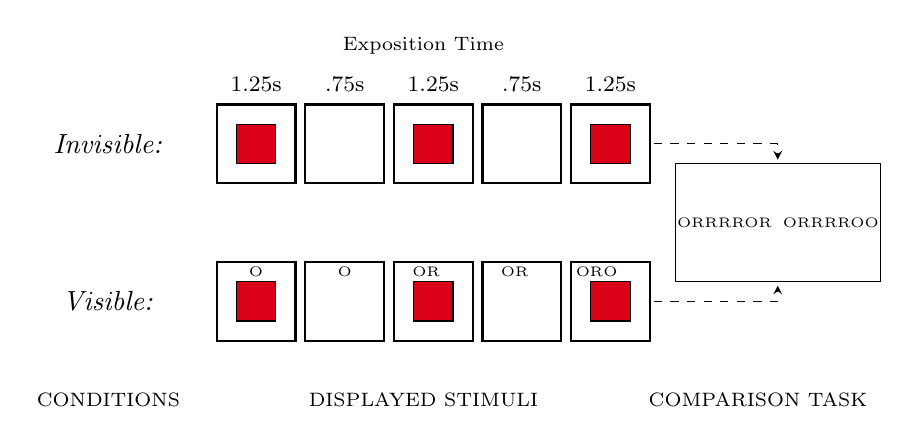
\begin{tikzpicture}[>=stealth, big/.style={scale = .5,
         % The shape:
         rectangle,
         % The size:
         minimum height=1cm,
         minimum width=2.5cm,
         % The border
         thick, draw=black,
         fill = white,
         % The filling
         % Font
         font=\itshape}]
         \begin{scope}[scale = .5, >=stealth]
            \node at (0,0.5) {\textit{Invisible:}};
            \node at (0,-3.5) {\textit{Visible:}};
            \foreach \x \y in {2.75/1.25s,5/.75s,7.25/1.25s,9.5/.75s,11.75/1.25s} {
                \draw [fill = white, draw = black, thick] (\x, -.5) rectangle (\x+2, 1.5);
            };
            \foreach \x \y in {2.75, 7.25, 11.75} {
                \draw [fill = rred, draw = black] (\x + .5, 0) rectangle (\x +1.5, 1);
            };
            \foreach \x \y in {2.75/1.25s,5/.75s,7.25/1.25s,9.5/.75s,11.75/1.25s} {
                \draw [fill = white, draw = black, thick] (\x, -4.5) rectangle (\x+2, -2.5);
                \draw node at (\x + 1, 2) {\footnotesize \y};
            };
            \draw node at (3.75,-2.75) {\tiny O};
            \draw node at (6,-2.75) {\tiny O};
            \draw node at (7.90,-2.75) {\tiny O};
            \draw node at (10.15,-2.75) {\tiny O};
            \draw node at (8.25,-2.75) {\tiny R};
            \draw node at (10.5,-2.75) {\tiny R};
            \draw node at (12.05,-2.75) {\tiny O};
            \draw node at (12.4,-2.75) {\tiny R};
            \draw node at (12.75,-2.75) {\tiny O};
            \foreach \x \y in {2.75, 7.25, 11.75} {
                \draw [fill = rred, draw = black] (\x + .5, -4) rectangle (\x +1.5, -3);
            };
            \draw node at (0,-6) {\scriptsize CONDITIONS};
            \draw node at (8,-6) {\scriptsize DISPLAYED STIMULI};
            \draw node at (16.5,-6) {\scriptsize COMPARISON TASK};
            \draw node at (8, 3) {\scriptsize Exposition Time};
	    \draw (14.4,-3) rectangle (19.6, 0);
	    \draw node at (15.65, -1.5) {\tiny ORRRROR};
	    \draw node at (18.35, -1.5) {\tiny ORRRROO};
            \draw [->, dashed] (13.85,0.5) -- (17,0.5) -- (17,.1);
            \draw [->, dashed] (13.85,-3.5) -- (17,-3.5) -- (17,-3.1);
         \end{scope}
      \end{tikzpicture}
\end{document}
